\chapter{}{Multi-Model Approach to Solar Irradiance Forecasting}

\subchapter{Overview}
A variety of solar irradiance forecasting techniques targeted at different forecast horizons have been developed using different input data based on the temporal variability of the forecast horizon, and the spatial scale of the input data. As shown in Fig.~\ref{fig:fig_variability}, intra-hour forecasts can follow from statistical time-series based models on surface measurements, or from tracking the cloud-motion observed with ground-based, all-sky cameras \cite{multimodal_intrahour}. Input data from satellite imagery tracking cloud motion has been shown to be useful for a forecast horizon between 30 minutes and 6 hours. For days-ahead forecast horizon, regional and global numerical weather prediction models, predicting the evolution of the atmospheric system have been shown to be more appropriate and accurate.

\begin{figure}[htbp]
    \begin{center}
    	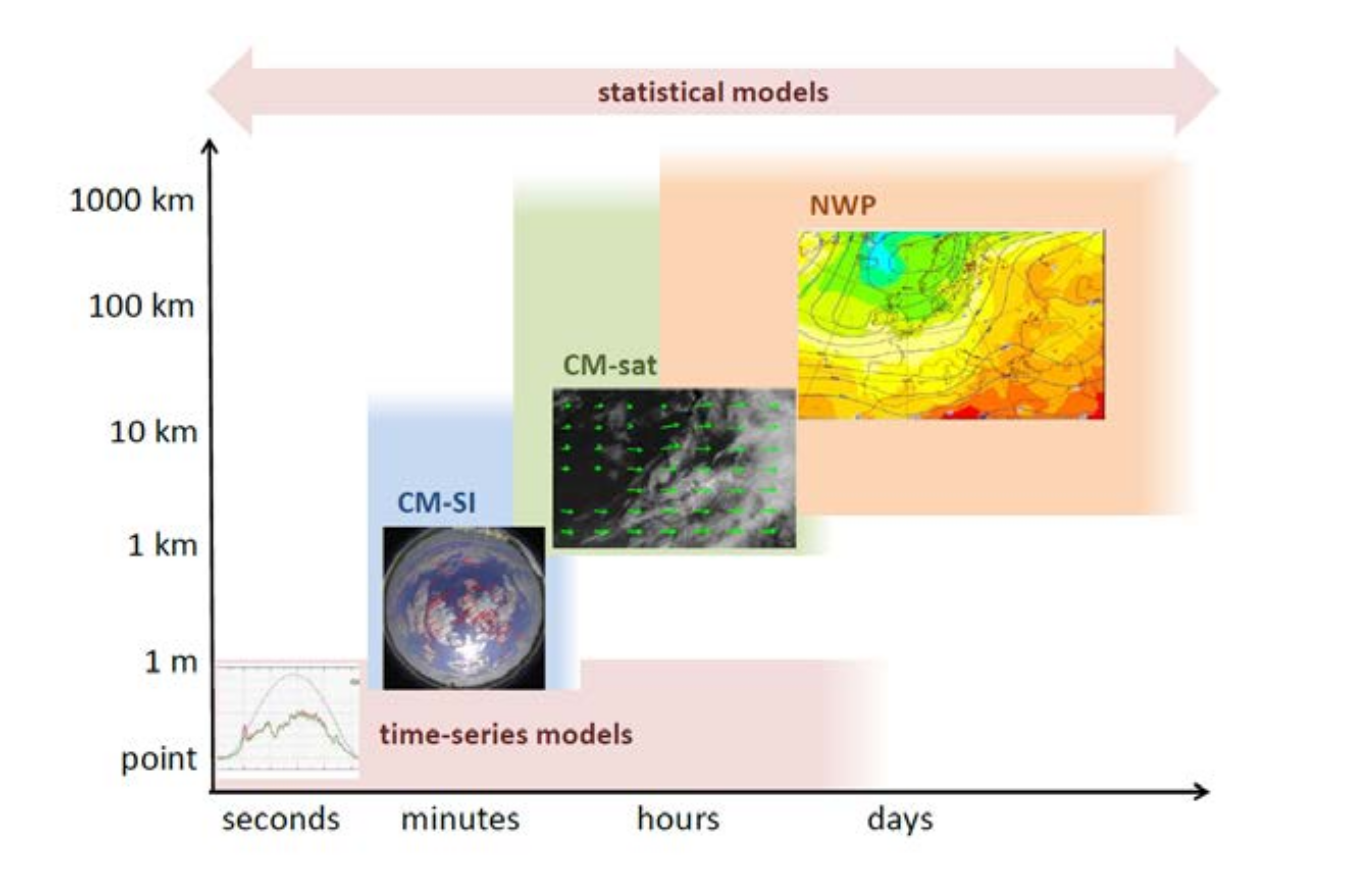
\includegraphics[width=0.75\textwidth]{chapter3/fig_variability.png}
    	\label{fig:fig_variability}
    	\caption{Input data based on varied spatial and temporal scales for solar forecasting \cite{multimodel_figure1}}
    \end{center}
\end{figure}

\par The numerical weather prediction models derive their initial conditions from different ground and airborne sensors from across the world, and based on equations describing the physical processes occurring in the atmosphere, forecast a parameter into the forecast horizon. The National Oceanic and Atmospheric Administration (NOAA) operates a variety of numerical weather prediction models with their spatial resolution ranging from approximately 10 km - 50 km, and their temporal reoslution typically being 1 hour or 3 hours, and which are normally updated every 6 hours \cite{multimodel_bestpractices}. 

\par In this work, we intended to forecast solar irradiance captured at the solar farm in Athens, Georgia for a forecast horizon of 24 hours. For this purpose, a mesoscale model which can predict parameters describing cloudiness such as \textit{North American Mesoscale (NAM)} Forecast System \cite{multimodel_nam} was used. Typical weather variables known to affect solar irradiance forecasting systems such as air temperature, geopotential height, cloud cover, visibility, wind speed, dew point temperature, air pressure, downwelling shortwave radiation flux, downwelling longwave radiation flux, and humidity were evaluated so as to gauge their effect on the solar irradiance predictions. This enabled a cut in computational cost of modeling and also led to an improvement in the performance of the model.

\par Downwelling shortwave radiation flux, synonymous with global horizontal irradiance (GHI) is measured by NWP models using columnar radiative transfer models (RTM). However, the direct output from the mesoscale models has shown severe deviations between forecasted and real irradiance \cite{multimodel_ghi}. While the usage of additional weather variables in machine learning models have shown to improve the post-processing of NWP models with site-specific information, one fact which has to be taken into consideration is that there is a significant variability in the GHI measured by the NWP models depending on the cloud conditions. As a matter of fact, Mathiesan et al \cite{multimodel_overpredict} found that the NAM forecast model tends to overpredict GHI in clear sky conditions by up to 40 percent.

\par There are multiple formulations which have been extensively discussed in literature which compute the irradiance metrics from environmental conditions such as cloud cover, and can be broadly classified into decomposition models and isotropic models. Using assumptions on solar geometry and transmittance, the former are used to estimate direct beam and diffuse irradiance. The latter are useful for approximating daily solar radiation reaching tilted surfaces. The irradiance metrics retrieved using either of these models can be used to empirically estimate global horizontal irradiance, which can further be used to correct the bias in GHI forecasts recorded by the NWP models. Such a bias correction can lead to an improvement in the post-processing of the input data for the machine learning models with respect to the solar irradiance observations from the solar farm.

\subsubchapter{Numerical Weather Prediction (NWP) Models}
Meteorological forecasts from Numerical Weather Prediction (NWP) models have successfully been employed for the purpose of solar forecasting. The making of a weather forecast revolves around assessing the current weather situation, assimilating observational information, and projecting this initial state into future based on the laws of thermodynamics. One of the major challenges faced in this process is determining the range of area to observe. As shown in Fig.~\ref{fig:figure1_variability}, the further the forecasting of the weather conditions, i.e, higher the forecast horizon, the wider is the range of area that needs to be observed. 

\par Multiple weather prediction models, both global and regional, depending on the spatial domain, are maintained by the National Oceanic and Atmospheric Administration (NOAA). Global Forecast System (GFS) is one of the widely-known global weather prediction models, while North America Mesoscale (NAM), Rapid Refresh (RAP), High Resolution Rapid Refresh (HRRR) are popular regional weather prediction models in the United States.

\begin{figure}[htbp]
    \begin{center}
    	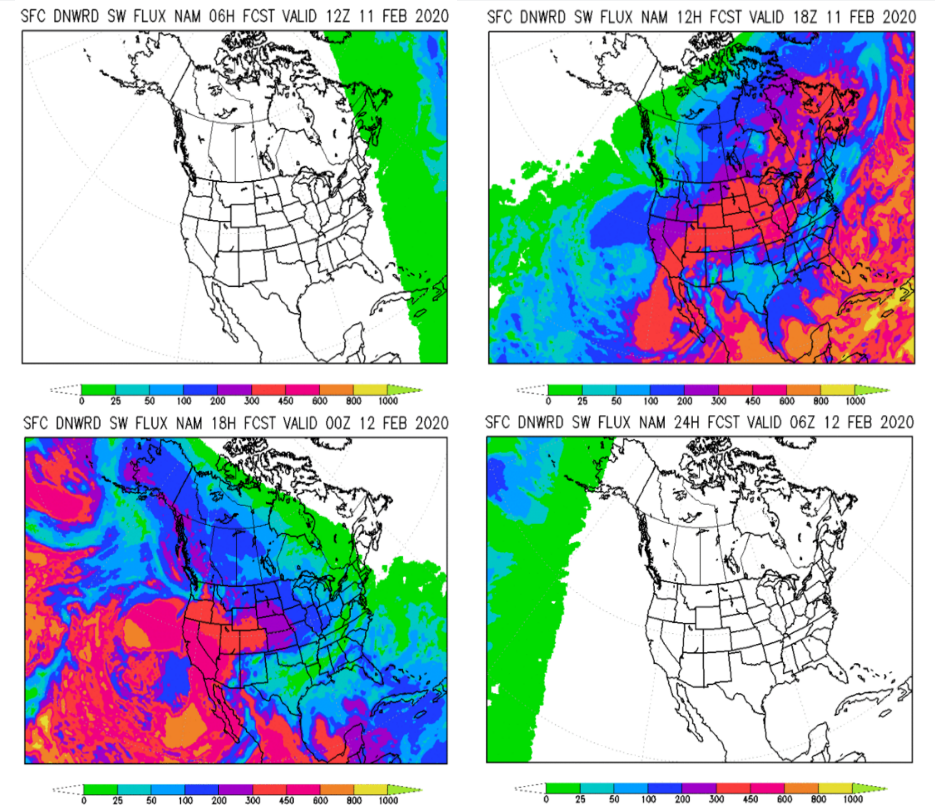
\includegraphics[width=0.85\textwidth]{chapter3/fig_nam_dswrf.png}
    	\label{fig:fig_nam_dswrf}
    	\caption{Downward Shortwave Radiation Flux parameter from NAM data for 06h forecast (top-left), 12h forecast (top-right), 18h forecast (bottom-left) and 24h forecast (bottom-right) \protect\footnote{NCEP Operational Graphics retrieved from \url{https://www.emc.ncep.noaa.gov/mmb/mmbpll/opsnam_archive/00z/}}}.
    \end{center}
\end{figure}

\par Write about NAM data with details

\subsubchapter{PVLIB Forecast Modeling}
Holmgrem et al \cite{pvlib_Holmgren2018} contributed to building pvlib-python\footnote{https://github.com/pvlib/pvlib-python} an open source, python-based tool, ported from the PVLIB MATLAB toolbox developed at the Sandia National Laboratories. This software provides a set of functions and classes for simulating the performance of the photovoltaic energy systems, with implementations of algorithms related to solar energy. In particular, the 'forecast' module contains objects to obtain weather forecast data from NOAA/NCEP/NWS models including the GFS, NAM, RAP, HRRR, and the NDFD, retrieved from the UNIDATA THREDDS servers, and convert that data into a PV power forecast. 

\par For our experiments, we created a NAM weather forecast dataset for the years of 2017 and 2018, retrieved from the NCEP servers. Meanwhile, pvlib-python retrieves NAM CONUS 12km resolution forecasts from THREDDS servers. The key difference between each of the datasets is that the former is a full complement of both the pressure level fields and surface-based fields, while the latter is a full complement of just the surface-based fields. In the forecast module, pvlib-python returns a dataset consisting of the following features: air temperature, wind speed, total clouds, low clouds, mid clouds, high clouds. 

\par To be able to use the pvlib-python functionalities, both the datasets were connected by mapping corresponding surface-level features. pvlib-python helps process the NAM data so as to compute irradiance metrics such as global horizontal irradiance (GHI), diffused horizontal irradiance (DHI) and direct normal irradiance (DNI) from the total cloud cover, using two techniques: Clearsky Scaling, Liu Jordan.


\subsubsection*{Clearsky Scaling}
Global horizontal irradiance can be measured with the help of a pyranometer on a horizontal surface, and thus, is typically, the most common type of irradiance measurement. Knowledge of the clear sky conditions, i.e. absence of clouds, is a key requirement for forecasting all the three irradiance metrics. Several parametric models have been proposed to compute these irradiance metrics from environmental conditions such as atmospheric turbidity, fractional sunshine, perceptible water vapor, etc. Ineichen et al \cite{pvlib_ineichen} formulated a model to compute Linke turbidity independent of the airmass, and global horizontal irradiance under clear sky conditions. Going by Larson et al's \cite{pvlib_larson} work, pvlib-python scales global horizontal irradiance on the basis of the total cloud cover. Furthermore, cloudy sky direct normal irradiance is determined based on the DISC \cite{pvlib_disc} model, and diffused horizontal irradiance is empirically formulated from global horizontal irradiance and direct normal irradiance thus calculated.

\subsubsection*{Liu-Jordan Method}
Decomposition models typically utilize only data pertaining to global radiation to estimate diffuse radiation from global solar irradiation data. They are based on the atmospheric effects in an isolated place, varying according to time of the year, season and climatic conditions \cite{pvlib_liujordan}. Liu et al proposed one of the earliest and simplest models of radiation, the Liu-Jordan model \cite{pvlib_liujordan2}, which presumes that diffuse radiation intensity is distributed uniformly over the whole sky, and helps estimate diffuse radiation on horizontal surfaces. It is also one of the more accurate among isotropic models for estimating diffused radiation on inclined surfaces \cite{pvlib_liujordan3}. This model helps determine direct normal irradiance, global horizontal irradiance from properties such as extraterrestrial flux, transmittance, and optical air mass number; and diffused horizontal irradiance from an empirical equation for diffuse radiation.

\subchapter{Methodology}
\subsubchapter{Data Collection and Preprocessing}
Lorem ipsum dolor sit amet, consectetur adipiscing elit, sed do eiusmod tempor incididunt ut labore et dolore magna aliqua. Ut enim ad minim veniam, quis nostrud exercitation ullamco laboris nisi ut aliquip ex ea commodo consequat. Duis aute irure dolor in reprehenderit in voluptate velit esse cillum dolore eu fugiat nulla pariatur. Excepteur sint occaecat cupidatat non proident, sunt in culpa qui officia deserunt mollit anim id est laborum.

\par Insert NAM data figure here.

\subsubsection*{Weather Forecasts}
\par Describe NAM data

\par Add subheading for feature selection in this section.


\subsubsection*{Temporal Features}
\par Contrast performance between Zach's features and current temporal features.

\par Note improvement in performance upon including temporal features as against persistance models.

\subsubsection*{Irradiance Observations}
\par Describe solar farm set up.

\par Insert image with pyranometers.

\subsubchapter{Multi Model}
\par Describe pyranometers and corresponding PVLIB modeling technique contrast


\subsubchapter{Geographic Extension}
\par Insert image with GA and corresponding grid extension

\subchapter{Experiment Setup}
Lorem ipsum dolor sit amet, consectetur adipiscing elit, sed do eiusmod tempor incididunt ut labore et dolore magna aliqua. Ut enim ad minim veniam, quis nostrud exercitation ullamco laboris nisi ut aliquip ex ea commodo consequat. Duis aute irure dolor in reprehenderit in voluptate velit esse cillum dolore eu fugiat nulla pariatur. Excepteur sint occaecat cupidatat non proident, sunt in culpa qui officia deserunt mollit anim id est laborum.

\subchapter{Results and Discussion}
Lorem ipsum dolor sit amet, consectetur adipiscing elit, sed do eiusmod tempor incididunt ut labore et dolore magna aliqua. Ut enim ad minim veniam, quis nostrud exercitation ullamco laboris nisi ut aliquip ex ea commodo consequat. Duis aute irure dolor in reprehenderit in voluptate velit esse cillum dolore eu fugiat nulla pariatur. Excepteur sint occaecat cupidatat non proident, sunt in culpa qui officia deserunt mollit anim id est laborum.

\begin{table}[h]
\begin{center}
    \caption{Sample Table 1}
    \begin{tabular}{ c c c c }
    	\toprule
    	col1 & col2 & col3 & col 4 \\
    	\midrule
    	\multirow{3}{4em}{Multiple row} & cell2 & cell3 & cell4\\ &
    	cell5 & cell6 & cell7 \\ &
    	cell8 & cell9 & cell10 \\
    	\midrule
    	\multirow{3}{4em}{Multiple row} & cell2 & cell3 & cell4 \\ &
    	cell5 & cell6 & cell7 \\ &
    	cell8 & cell9 & cell10 \\
    	\bottomrule
    \end{tabular}
\end{center}
\end{table}

Lorem ipsum dolor sit amet, consectetur adipiscing elit, sed do eiusmod tempor incididunt ut labore et dolore magna aliqua. Ut enim ad minim veniam, quis nostrud exercitation ullamco laboris nisi ut aliquip ex ea commodo consequat. Duis aute irure dolor in reprehenderit in voluptate velit esse cillum dolore eu fugiat nulla pariatur. Excepteur sint occaecat cupidatat non proident, sunt in culpa qui officia deserunt mollit anim id est laborum.

\newpage